% Imported from algorithms/reference-conditioning/README.md
\chapter{多模态参考控制}\label{seedance-m07}
\moduleinfo{M07}{基础方法与机制解释}{\hyperref[src-phantom]{\texttt{phantom}}、\hyperref[src-long-context-tuning]{\texttt{long-context-tuning}}、\hyperref[src-vincie]{\texttt{vincie}}、\hyperref[src-vincie-next]{\texttt{vincie-next}}、\hyperref[src-wan-2.1]{\texttt{wan-2.1}}、\hyperref[src-phantom-code]{\texttt{phantom-code}}}

表示已有以后，再沿总图的参考支路看：素材怎样成为可读取条件，目标主干怎样使用它。

把一张图作为参考，究竟是在参考什么？可能是人物身份，也可能只是衣服、构图或风格；动作视频还可能只负责相机运动。先把这个条件含义说清楚，再讨论编码。否则将素材全部拼接，连模型应该保留哪一部分都还没有定义。

例如人物 A 的脸来自图片，运动来自视频，音色来自音频。三者对目标的约束不同，绑定也要分别保留。若只传内容而不传用途，动作参考中的服装和背景、声音参考中的音乐，都可能一起进入结果。

\section{低层细节与高层语义各有什么用}\label{seedance-m07-ux4f4eux5c42ux7ec6ux8282ux4e0eux9ad8ux5c42ux8bedux4e49ux5404ux6709ux4ec0ux4e48ux7528}

对一张参考图，可以同时保留两类表示。VAE 潜变量保存纹理、颜色和局部结构，图像语义编码器再提供主体类别、外观概念及较抽象的身份信息。下面把它们写成两条条件路径：

\begin{figure}
\centering
\pandocbounded{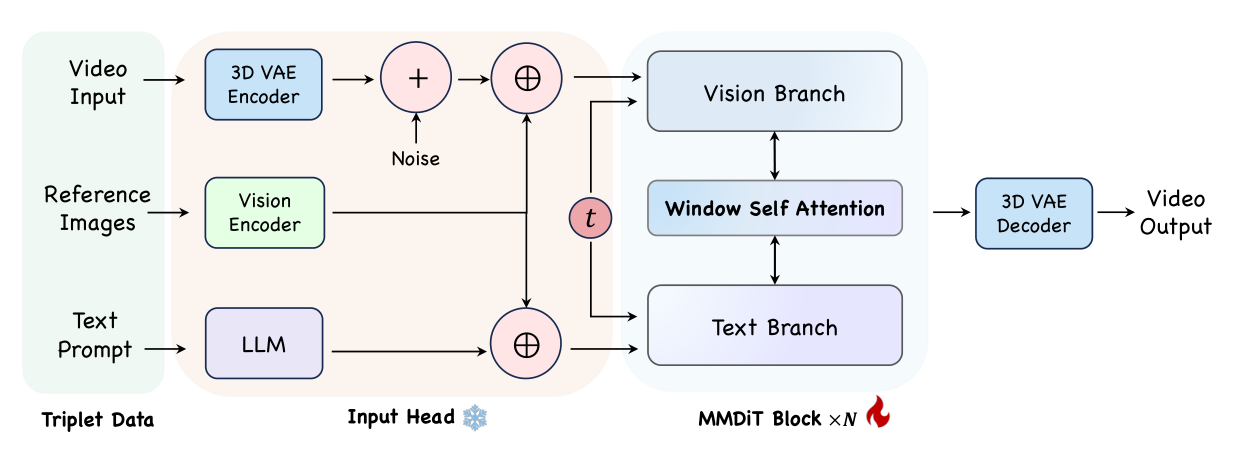
\includegraphics[keepaspectratio,alt={参考图细节与语义分别进入生成模型 （论文示意，来源：phantom）}]{assets/seedance/figures/subject-reference.png}}
\caption{参考图细节与语义分别进入生成模型 （论文示意，来源：phantom）}
\end{figure}

两条路径并不是越强越好。细节过强时，模型可能连姿态和背景都复制，视角、动作难以变化；语义过强时，又可能只剩“穿蓝衣的人”，具体长相和纹理丢掉了。因此可用条件 dropout、多视角配对和动作对照，检查每条路径到底保留了什么。

在窗口注意力中，还可以让参考信息进入多个窗口，使局部视频 token 都有机会读取主体信息。输入数量可变不代表开销不变，参考如何重复、压缩和聚合都需要明确。

\section{素材绑定应成为显式数据}\label{seedance-m07-ux7d20ux6750ux7ed1ux5b9aux5e94ux6210ux4e3aux663eux5f0fux6570ux636e}

每份素材至少记录 \codepath{asset_id}、\codepath{modality}、\codepath{role}、\codepath{subject_id}、\codepath{shot_ids}、\codepath{time_range} 和 \codepath{priority}。role 可以区分身份、外观、动作、相机、布局、风格与音色。

有了绑定，冲突才有地方处理。比如图片指定红外套，动作视频中的人却穿蓝外套：若视频只负责动作，它的服装信息就不应与图片争权重；若要求综合，先规定哪项优先。否则同一目标同时收到互斥条件，结果很难解释。

白模也属于参考条件。它可以先渲染为二维帧序列，或者额外提供 depth、normal、pose 和 camera 参数；不必天然使用原生 mesh encoder。显式结构条件通常更容易定位几何约束，但需要同步的训练数据和坐标定义。

\section{怎样在已有基座上增加参考能力}\label{seedance-m07-ux600eux6837ux5728ux5df2ux6709ux57faux5ea7ux4e0aux589eux52a0ux53c2ux8003ux80fdux529b}

若在现有基座上逐步加功能，可以先保留原 VAE、patch 与文本接口，只增一条参考读取路径。令目标视频给 query，参考给 key/value，门控控制新增残差，得到：

\[
\Delta h_v=\operatorname{Attn}(Q_v,K_r,V_r),
\qquad h'_v=h_v+g\Delta h_v.
\]

这一步的计算含义比较直接：每个视频位置问一个问题，参考记忆提供可以读取的内容，最后把读到的增量加回视频状态。是否使用某份参考，再由它与镜头、角色及时间的绑定来限制。这样参考怎样进入主干，就不再只是一句“加入参考条件”。

参考图先经过编码、投影与定额池化，得到 \codepath{B,R,d_ref} 的参考记忆。role、subject 和时间信息随 token 一起进入；视频 query 通过绑定 mask 读取适用的参考。

这个mask只能使用推理时真正可获得的信息：镜头允许的主体集合、布局、源视频跟踪或预测区域。纯噪声目标的空间query没有已知subject ID；无空间归属时先做镜头级粗筛，通过主体embedding和训练学习对应，不能假设一个标签已经解决多人空间绑定。

初始化也要沿计算图看。门控 \(g\) 从零开始，新投影正常作小方差初始化，先让支路能够在不扰动主干的情况下接入；若 gate 与整个支路同时全零，起始梯度可能被相互挡住。先训练参考支路，再用对照判断是否需要主干 LoRA 或有限解冻。

这里讨论的是独立 adapter。MMDiT 的窗口动态注入有自己的连接方式，不能把两种实现都叫“参考模块”就混用。应先看基座原本接收什么，再看手里的训练数据能监督哪一种关系。

\section{文件数量与 token 预算是两种容量}\label{seedance-m07-ux6587ux4ef6ux6570ux91cfux4e0e-token-ux9884ux7b97ux662fux4e24ux79cdux5bb9ux91cf}

假设视频有 \(N_v\) 个 token，参考编码后有 \(R\) 个 token。直接把参考拼进完整自注意力，新增连接规模约为：

\[
(N_v+R)^2-N_v^2=2N_vR+R^2.
\]

独立交叉注意力可以避免一部分不必要的参考内部交互，但仍有约 \(N_vR\) 的连接。几十个文件经过编码，可能变成远超几十个 token 的条件序列。

因此可以按镜头检索有效参考，再按优先级分配预算。例如先试总计 1024 个参考 token，比较它与更高预算的质量差异。这个数字只是试验起点，不能保证足以表示大量人物、精细 logo 和音色。

压成较少 token 后，细小部件也可能一起丢失。因此还要保存实际读取了哪些素材、怎样裁剪、保留多少 token，以及哪些被截断。用户提供了参考，与模型实际使用了参考，在这里仍是两个不同事实。

\section{参考训练数据怎样避免复制}\label{seedance-m07-ux53c2ux8003ux8badux7ec3ux6570ux636eux600eux6837ux907fux514dux590dux5236}

数据配对同样影响模型学到什么。从目标视频截一帧作参考，背景和姿态也高度相同，复制就可能把损失降下来。换成跨片段的同主体配对，才更接近保持身份、改变动作与环境的目标。不过相似 embedding 不能直接证明同一主体，错配会污染身份监督。

评测应同时改变参考数、主体数、背景、动作幅度和参考冲突程度，分别检查身份、服装、动作、相机和背景泄漏。先证明两到四份参考比最佳单参考更有帮助，再扩大数量，才能分清模型真正使用了多参考，还是接口仅仅接受了更多文件。

\section{从极简代码到真实实现}\label{seedance-m07-ux4eceux6781ux7b80ux4ee3ux7801ux5230ux771fux5b9eux5b9eux73b0}

参考支路的最小逻辑，是视频生成 query、参考生成 key/value，再按绑定 mask 限制读取：

\begin{verbatim}
q = video_projection(video)
k, v = reference_key(reference), reference_value(reference)
delta = attention(q, k, v, allowed_reference_mask)
output = video + gate * delta
\end{verbatim}

\hyperref[code-reference-adapter]{reference\_adapter.py} 保留了零门控和布尔绑定，假设每个 query 至少有一个有效参考。真实参考编码与采样看 \href{https://github.com/Phantom-video/Phantom/blob/bd84b602dcc949e23c89cbbf266b6f5975f2f025/phantom_wan/subject2video.py}{Phantom-Wan subject2video}，主干注入看 \href{https://github.com/Phantom-video/Phantom/blob/bd84b602dcc949e23c89cbbf266b6f5975f2f025/phantom_wan/modules/model.py}{Phantom-Wan model}。该固定版提供推理，训练代码仍未发布，不能把示例支路当成其训练复现。
